%%% LaTeX Template: Article/Thesis/etc. with colored headings and special fonts
%%%
%%% Source: http://www.howtotex.com/
%%% Feel free to distribute this template, but please keep to referal to http://www.howtotex.com/ here.
%%% February 2011

%%%%% Preamble
\documentclass[10pt,a4paper]{article}

\usepackage[T1]{fontenc}
\usepackage[bitstream-charter]{mathdesign}

\usepackage[latin1]{inputenc}							% Input encoding
\usepackage{amsmath}		% Math
							
\usepackage{graphicx}

\usepackage{xcolor}
\definecolor{bl}{rgb}{0.0,0.2,0.6} 


\usepackage{sectsty}
\usepackage[compact]{titlesec} 
\allsectionsfont{\color{bl}\scshape\selectfont}

%%%%% Definitions
% Define a new command that prints the title only
\makeatletter							% Begin definition
\def\printtitle{%						% Define command: \printtitle
    {\color{bl} \centering \huge \sc \textbf{\@title}\par}}		% Typesetting
\makeatother							% End definition

\title{Z Donusumu \\ 
		\large \vspace*{-10pt} Teori ve Uygulamasi\vspace*{10pt}}

% Define a new command that prints the author(s) only
\makeatletter							% Begin definition
\def\printauthor{%					% Define command: \printauthor
    {\centering \small \@author}}				% Typesetting
\makeatother							% End definition

\author{%
	NAZIM YILDIZ \\
	nazimyildiz90@gmail.com \\
	\vspace{20pt}
	}

% Custom headers and footers
\usepackage{fancyhdr}
	\pagestyle{fancy}					% Enabling the custom headers/footers
\usepackage{lastpage}	
	% Header (empty)
	\lhead{}
	\chead{}
	\rhead{}
	% Footer (you may change this to your own needs)
	\lfoot{\footnotesize \texttt{nazimyildizblog.com} - Template}
	\cfoot{}
	\rfoot{\footnotesize page \thepage\ of \pageref{LastPage}}	% "Page 1 of 2"
	\renewcommand{\headrulewidth}{0.0pt}
	\renewcommand{\footrulewidth}{0.4pt}

% Change the abstract environment
\usepackage[runin]{abstract}			% runin option for a run-in title
\setlength\absleftindent{30pt}		% left margin
\setlength\absrightindent{30pt}		% right margin
\abslabeldelim{\quad}						% 
\setlength{\abstitleskip}{-10pt}
\renewcommand{\abstractname}{}
\renewcommand{\abstracttextfont}{\color{bl} \small \slshape}	% slanted text


%%% Start of the document
\begin{document}
%%% Top of the page: Author, Title and Abstact
\printtitle 

\printauthor

\begin{abstract}
Bu calismada faz farkli sinus denkleminin Z donusumu bulunarak herhangi bir mikrodenetleyicide kosturulabilinmesi icin izlenmesi gereken yol haritasi verilmistir.
\end{abstract}

%%% Start of the 'real' content of the article, using a two column layout
\section{Z Donusumu Teori}
Z donusumu dijital kontrol sistemlerinde kullanilan, islemcilerimizde elde ettigimiz denklemleri kosturabilmemiz icin kullandigimiz bir aractir. Ornegin 
zamana bagli herhangi bir fonksiyonu $sin(w \times t + \phi)$, $cos(w \times t + \phi)$, ... yada s-ortaminda transfer fonksiyonunu elde ettigimiz herhangi bir esitligi kolayca islemcilerde kosturabiliriz.

Z donusumu icin denklem-\ref{equ:z_formul}'de verilen seri toplam esitligi kullanilir.
\begin{equation} \label{equ:z_formul} 
	\begin{split}
	F(z) 	&= \sum_{n = 0}^{\infty} f(n \times T_{s}) \times z^{-n}
	\end{split}					
\end{equation}

$f(t) = V \times e ^ {-a \times t}$ olmak uzere, $T_s$ periyodu ile ornekleme yapildiginda ayrik zaman denklemi $f(n \times T_s) = V \times e ^ {-a \times n \times T_s}$ seklinde yazilir. Bu esitlige geometrik seri acilim formulu uygulandiginda denklem-\ref{equ:seri_sonuc} elde edilir.

\begin{equation} \label{equ:seri_sonuc} 
\begin{split}
	F(z) 	&= V \times \frac{1}{1 - e ^ {-a \times T} \times z^{-1}}
\end{split}					
\end{equation}

\subsection{Faz Farkli Sinus Z Donusumu}
Faz farki $\phi$ ve acisal frekansi w olan sinus denklemi $f(t) = sin(w \times t + \phi)$ seklinde yazilacak olursa, bu ifadeyi ayrik zamandaki karsiligini $t = n \times T_s$ yazarak $f(n \times T_s) = sin(w \times n \times T_s + \phi)$ seklinde elde ederiz. \newline 

\begin{equation} \label{equ:euler} 
\begin{split}
	e^{j \times w \times t} 	&= cos(w \times t) + j \times sin(w \times t) \\
	e^{-j \times w \times t} &= cos(w \times t) - j \times sin(w \times t) \\
	sin(w \times t) &= \frac{e^{j \times w \times t} - e^{-j \times w \times t}}{2j} \\
\end{split}					
\end{equation}
Elde edilen $f(n \times T_s)$ \footnote{$f(n \times t) = f[n] seklinde gosterilir.$} ayrik sinus denklemi, denklem-\ref{equ:euler}'deki euler esitligi kullanilarak ayrik sinus denklemi ustel formda elde edilir ve denklem-\ref{equ:seri_sonuc}'deki formul kullanilarak Z donusumu bulunabilir.

%%Sinus fark denklemi elde ediliyor
\begin{equation} \label{equ:ayrik_sin_euler} 
\begin{split}
	f[n] &= \frac{e^{j \times (w \times n \times T_s + \phi)} - e^{-j \times (w \times n \times T_s + \phi)}}{2j} \\
\end{split}					
\end{equation}
Faz farkli sinus denkleminin dijital karsiligi adim adim asagidaki gibi elde edilir.
\begin{equation} \label{equ:ayrik_sin_z_don1} 
\begin{split}
	f[n] &= \frac{1}{2j} \times  (e^{j \phi} \times e^{j \times w \times n \times T_s} - e^{-j\phi} \times e^{-j \times w \times n \times T_s})\\
\end{split}					
\end{equation}
Burada $e^{j \times \phi}$ ifadelerini katsayi gibi dusunebiliriz cunki bunlar n degiskenine bagli degiller. Diger n bagli 2 ustel ifadeyi ayri ayri Z donusumunu alip sonuca gidebiliriz.
\begin{equation} \label{equ:ayrik_sin_z_don2} 
\begin{split}
	F(z) &= \frac{1}{2j} \times (\frac{e^{j \phi}}{1 - e^{j \times w \times T_s}\times z^{-1}} - \frac{e^{-j \phi}}{1 - e^{-j \times w \times T_s}\times z^{-1}}) \\
	F(z) &= \frac{1}{2j} \times (\frac{e^{j \phi} - e^{-j \phi} + e^{j \times w \times T_s} \times e^{-j \phi} \times z^{-1} - e^{-j \times w \times T_s} \times e^{j \phi} \times z^{-1}}{1 - e^{-j \times w \times T_s} \times z^{-1} - e^{j \times w \times T_s} \times z^{-1} + z^{-2}}) \\
	F(z) &= \frac{sin(\phi) + sin(w \times T_s - \phi) \times z^{-1}}{1 - 2 \times cos(w \times T_s) \times z^{-1} + z^{-2}}
\end{split}					
\end{equation}
Burada;
\begin{itemize}
	\item w : Acisal frekansi, $2 \times \pi \times f$
	\item $T_s$ : Ornekleme periyodu
	\item $\phi$ : Faz acisini
\end{itemize}
belirtmektedir.
\subsection{Fark Denkleminin Elde Edilmesi}
Denklem-\ref{equ:ayrik_sin_z_don2}'da faz farkli sinus icin Z donusumu elde edildi. Bu ifadeyi bu haliyle islemcide kodlanamaz tekrar ayrik zaman ortamina gecmemiz gerekir. Bu asamada tercih edebilecegimiz 3 yontem var ve ben bu yontemler arasindan direk gercekleme yontemini kullanacagim. Adim adim cozum asagidaki gibidir.
\begin{equation} \label{equ:ayrik_sin_z_don3} 
\begin{split}
	F(z) &= \frac{O(z)}{I(z)}	\\
	F(z) &= \frac{O(z)}{R(z)} \times \frac{R(z)}{I(z)}	\\
	O(z) &= R(z) \times sin(\phi) + R(z) \times z^{-1} \times sin(w \times T_s - \phi) \\
	I(z) &= R(z) - R(z) \times z^{-1} \times 2cos(w \times T_s) + R(z) \times z^{-2} \\
	R(z) &= I(z) + R(z) \times z^{-1} \times 2cos(w \times T_s) - R(z) \times z^{-2} \\
\end{split}					
\end{equation}
Z degiskenine bagli olarak giris ve cikis arasindaki baginti yukaridaki gibi elde edildi. Burada R(z)'i giris ile cikis arasindaki baglanti noktasi olarak dusunebilirsiniz. Son adim olarak bu denklemlerin ayrik zamandaki karsiligini $z^{-x}$ degerlerinin ornek geciktirme operatoru oldugu bilgisini kullanarak denklem-\ref{equ:ayrik_sin_z_don4}'deki gibi elde ederiz.
\begin{equation} \label{equ:ayrik_sin_z_don4} 
\begin{split}
	o[n] &= r[n] \times sin(\phi) + r[n - 1] \times sin(w \times T_s - \phi) \\
	r[n] &= i[n] + r[n - 1] \times 2cos(w \times T_s) - r[n - 2] \\
\end{split}					
\end{equation}
Denklem-\ref{equ:ayrik_sin_z_don4} icin blok sema resim-\ref{fig:blok_sema} de verilmistir.
\begin{figure}
\centering
	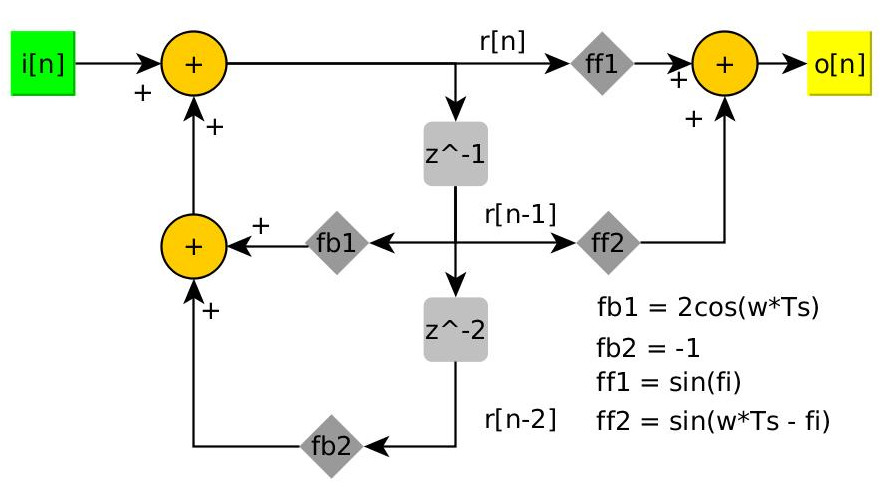
\includegraphics[width=0.7\linewidth]{blok_sema_kirpildi}
	\caption{Faz farkli sinus fark denklemi blok semasi}
\label{fig:blok_sema}
\end{figure}

\section{Uygulama}
Uygulama ciktilara buraya eklencek.

\end{document}